\documentclass{article}
\usepackage[utf8]{inputenc}
\usepackage[margin=2.6cm]{geometry}
\usepackage{float}
\usepackage{graphicx}
\usepackage{rotating}
\usepackage{caption}
\usepackage{subcaption}
\usepackage[round]{natbib}
\usepackage{setspace}
\onehalfspacing
\usepackage{tikz}
\usetikzlibrary{arrows,automata,positioning}

\title{The interplay of resource acquisition and sharing dynamics explains the diversity of female human reproductive allocative decisions.
\\
Registered Report}
\author{Pablo J. Varas Enriquez, Monique Bogerhoff Mulder, Heidi Colleran, Dieter Lukas*\\\\
* No special order of authors}
\date{\today}

\begin{document}

\maketitle

\tableofcontents

\section{Problem Formulation}

There are many developmental paths an individual can follow through its life cycle, which is the basis of the diversity seen across the tree of life. The diversity of reproductive schedules can go from a couple to thousands offspring (e.g. eastern hemlock vs rain moth \citep{tindale1932revision,van2017lifetime} and mortality ones from lifespans of days to thousands of years (e.g. hairyback vs patagonian cypress \citep{balsamo1988life,lara19933620}). The different life cycles have usually been related to the limited resources an individual posses in its environment and how it allocates them \citep{stearns2000life}. Humans pose an interesting case regarding its life cycle due to the short reproductive period in comparison to their long lifespan, framed within long juvenile and post-reproductive stages \citep{kaplan2000theory}. Within these boundaries, humans present a high diversity of life cycles with populations where life spans are long and their reproductive output is low (e.g. post-demographic transition Japan \citep{de2017maximum}) while others have short lifespans and high reproductive output (e.g. pygmies populations \citep{migliano2007life}).  The boundaries of the different life stages, and the variability of longevity, reproductive timing and output, are influenced by individual reproductive allocative decisions (e.g. age at menarche, number of offspring, age at last reproduction). The diversity in female human reproductive allocative decisions has been associated with resource availability, specially in terms of longevity \citep{kaplan2003embodied}; while for fertility the relationship is more complex \citep{mulder1998demographic,sear2016understanding}. Additionally, sharing resources has been proposed as a way to understand the different life cycles among female human populations. Here, the presence or different members of a population in the social network of an individual have been associated with different female reproductive allocative decisions \citep{sear2011much}. Examples can be found in literature related to cooperative breeding, sibling competition, female conflict, among others \citep{ivey2000cooperative,nitsch2013elder,mace2012female}.However, both frameworks have not been able, separately, to explain what drives the diversity of female human reproductive allocative decisions. The interplay between the resources an individual acquisition and its sharing dynamics may be key to understand how the female human life cycle has evolved and diversified. Hence,  this project aims to develop a theoretical framework to describe how the interplay of resource acquisition and their sharing across the social network may be key to understand female reproductive allocative decisions. More specifically, the model would allow to analyse which scenarios might vary the timing of life stage transitions, longevity, and reproductive timing and output of individuals, and their fitness, ultimately.
\\\\
The model will be developed in an agent-based model framework, considering that the aims are a) to observe the ages of transition between stages, longevity, and reproductive behaviour (i.e. reproductive output and timing) that emerge in scenarios with different resource productivity and sharing dynamics, and b) calculate fitness differences associated with the different life cycles that emerge in the different scenarios. Therefore, the model will be described using an ODD (Overview, Design concepts, Details) protocol, as an standardised way to clarify the scope, assumptions, and parameters used to answer our questions \citep{grimm2006standard,grimm2020odd}.

\section{Model description}

\subsection{Purpose}

The female human life cycle is characterised by a long lifespan, within which there is usually a short reproductive period in between long juvenile and post-reproductive stages. The boundaries of the reproductive period, and the frequency at which births occur during this period, are influenced by individual reproductive allocative decisions. Previous work has linked reproductive allocative decisions to the amount of resources available to an individual in its environment or the availability of a network of potential helpers, but how the interplay of both of them change reproductive allocative decisions of an individual, and its life cycle as consequence, remains unclear. Here we will develop a theoretical framework to understand how the interplay of resource acquisition and their sharing across the social network influence female reproductive allocative decisions. More specifically, the model would allow identify which scenarios vary the timing of life stage transitions, longevity, and reproductive timing and output of individuals, and their fitness, ultimately. A graphical explanation can be seen in Fig. \ref{fig:1}

\begin{figure}[H]
    \centering
    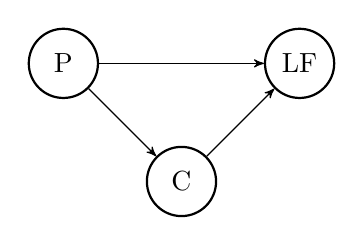
\begin{tikzpicture}[->,>=stealth',auto,thin]
\tikzstyle{every state}=[fill=white,shape=circle,draw,thick,text=black, text centered, text width=0.5cm, align=center]

\node[state]		(A)              {P};
\node[state]		(B) [right of=A,node distance=1.5cm,draw=none,fill=none] {};
\node[state]		(C) [below of=B,node distance=1.5cm] {C};
\node[state]		(D) [right of=B,node distance=1.5cm] {LF};

\path
(A) edge (D)
(A) edge (C)
(C) edge (D)
;
    \end{tikzpicture}
%
    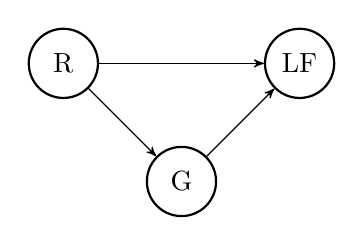
\begin{tikzpicture}[->,>=stealth',auto,thin]
\tikzstyle{every state}=[fill=white,shape=circle,draw,thick,text=black, text centered, text width=0.5cm, align=center]

\node[state]		(A)              {R};
\node[state]		(B) [right of=A,node distance=1.5cm,draw=none,fill=none] {};
\node[state]		(C) [below of=B,node distance=1.5cm] {G};
\node[state]		(D) [right of=B,node distance=1.5cm] {LF};

\path
(A) edge (D)
(A) edge (C)
(C) edge (D)
;
    \end{tikzpicture}

    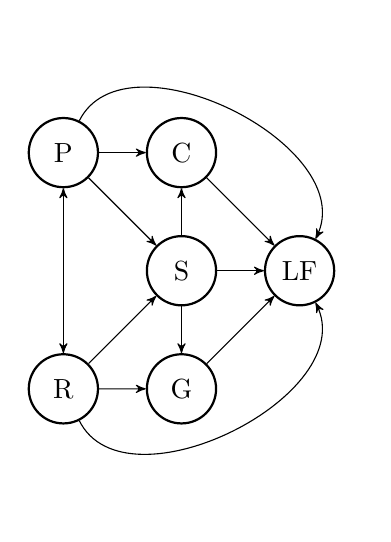
\begin{tikzpicture}[->,>=stealth',auto,thin]
\tikzstyle{every state}=[fill=white,shape=circle,draw,thick,text=black, text centered, text width=0.5cm, align=center]

\node[state]		(A)              {P};
\node[state]		(B) [right of=A,node distance=1.5cm] {C};
\node[state]		(C) [below of=B,node distance=1.5cm] {S};
\node[state]		(D) [below of=A,node distance=3cm] {R};
\node[state]        (E) [below of=C,node distance=1.5cm] {G};
\node[state]        (F) [right of=C,node distance=1.5cm] {LF};

\path
(A) edge (B)
(A) edge (C)
(A) edge[<->] (D)
(A) edge[bend right=-90, min distance=1cm] (F)
(B) edge (F)
(C) edge (B)
(C) edge (E)
(C) edge (F)
(D) edge (C)
(D) edge (E)
(D) edge[bend left=-90, min distance=1cm] (F)
(E) edge (F)
;
    \end{tikzpicture}
    \caption{Caption}
    \label{fig:1}
\end{figure}

For the purpose of this model, the life cycle of an individual will be described by the time spent across five discrete stages (i.e. infant, juvenile, adult, reproductive-career, post-reproductive) and the number of surviving offspring until sexual maturity (i.e. lifetime reproductive success). Therefore, reproductive allocative decisions will be understood as the key events that define the individual life cycle, including the timing of each life stage transition, longevity, and reproductive timing and output. Resource acquisition in the model will be related to resource production and consumption, while sharing will be related to the giving and receiving dynamics an individual is subject to. A graphical representation can be seen in Fig. \ref{fig:2}.


\begin{sidewaysfigure}
\begin{figure}[H]
    \centering
     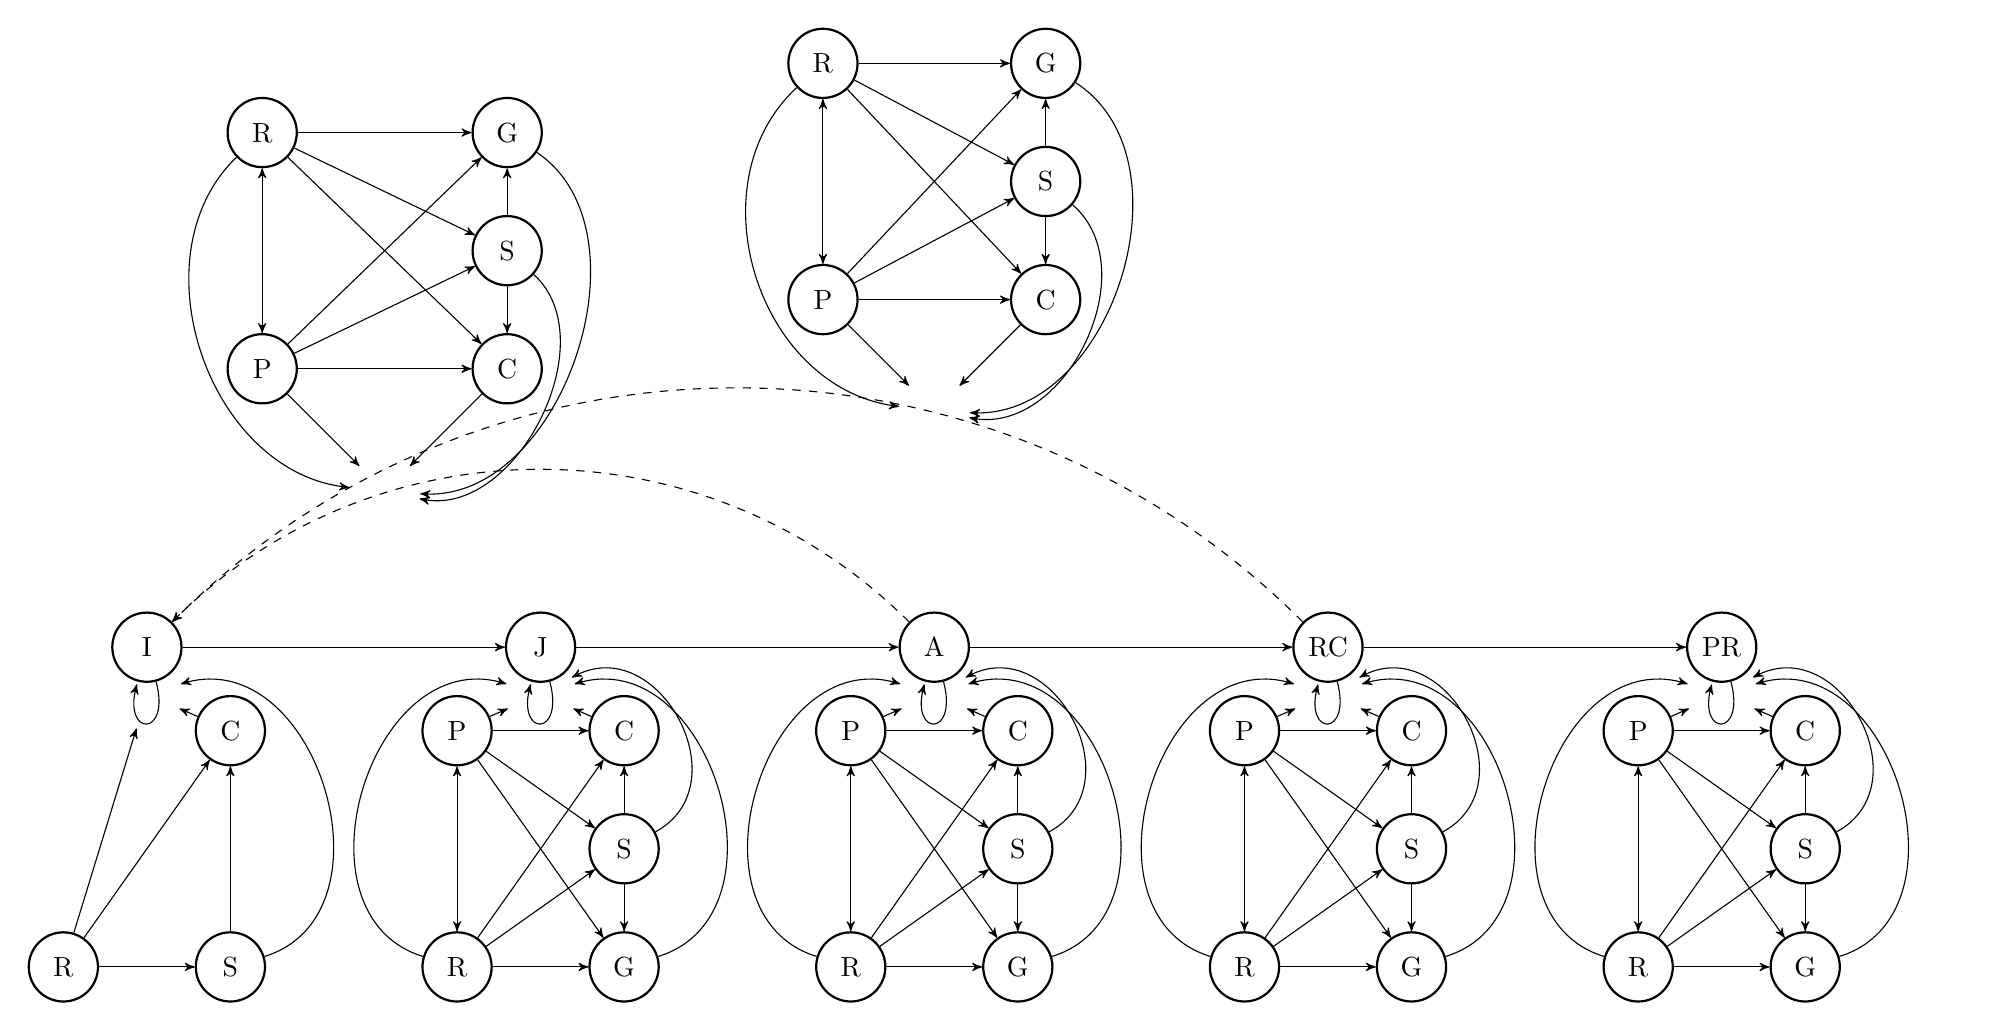
\begin{tikzpicture}[->,>=stealth',auto,thin]
\tikzstyle{every state}=[fill=white,shape=circle,draw,thick,text=black, text centered, text width=0.5cm, align=center]

\node[state]		(A)              {I};
\node[state]		(B) [below of=A,node distance=0.6cm,draw=none,fill=none] {};
\node[state]		(C) [below left of=A,node distance=1.5cm,draw=none,fill=none] {};
\node[state]		(D) [below of=C,node distance=1.5cm,draw=none,fill=none] {};
\node[state]        (E) [below of=D,node distance=1.5cm] {R};
\node[state]        (F) [below right of=A,node distance=1.5cm] {C};
\node[state]		(G) [below of=F,node distance=1.5cm,draw=none,fill=none] {};
\node[state]        (H) [below of=G,node distance=1.5cm] {S};
\node[state]		(I) [right of=A, node distance=5cm]             {J};
\node[state]		(J) [below of=I,node distance=0.6cm,draw=none,fill=none] {};
\node[state]		(K) [below left of=I,node distance=1.5cm] {P};
\node[state]		(L) [below of=K,node distance=1.5cm,draw=none,fill=none] {};
\node[state]        (M) [below of=L,node distance=1.5cm] {R};
\node[state]        (N) [below right of=I,node distance=1.5cm] {C};
\node[state]		(O) [below of=N,node distance=1.5cm] {S};
\node[state]        (P) [below of=O,node distance=1.5cm] {G};
\node[state]		(Q) [right of=I, node distance=5cm]             {A};
\node[state]		(R) [below of=Q,node distance=0.6cm,draw=none,fill=none] {};
\node[state]		(S) [below left of=Q,node distance=1.5cm] {P};
\node[state]		(T) [below of=S,node distance=1.5cm,draw=none,fill=none] {};
\node[state]        (U) [below of=T,node distance=1.5cm] {R};
\node[state]        (V) [below right of=Q,node distance=1.5cm] {C};
\node[state]		(W) [below of=V,node distance=1.5cm] {S};
\node[state]        (X) [below of=W,node distance=1.5cm] {G};
\node[state]		(Y) [right of=Q, node distance=5cm]             {RC};
\node[state]		(Z) [below of=Y,node distance=0.6cm,draw=none,fill=none] {};
\node[state]		(AA) [below left of=Y,node distance=1.5cm] {P};
\node[state]		(BB) [below of=AA,node distance=1.5cm,draw=none,fill=none] {};
\node[state]        (CC) [below of=BB,node distance=1.5cm] {R};
\node[state]        (DD) [below right of=Y,node distance=1.5cm] {C};
\node[state]		(EE) [below of=DD,node distance=1.5cm] {S};
\node[state]        (FF) [below of=EE,node distance=1.5cm] {G};
\node[state]		(GG) [right of=Y, node distance=5cm]             {PR};
\node[state]		(HH) [below of=GG,node distance=0.6cm,draw=none,fill=none] {};
\node[state]		(II) [below left of=GG,node distance=1.5cm] {P};
\node[state]		(JJ) [below of=II,node distance=1.5cm,draw=none,fill=none] {};
\node[state]        (KK) [below of=JJ,node distance=1.5cm] {R};
\node[state]        (LL) [below right of=GG,node distance=1.5cm] {C};
\node[state]		(MM) [below of=LL,node distance=1.5cm] {S};
\node[state]        (NN) [below of=MM,node distance=1.5cm] {G};
\node[state]		(OO) [above left of=I, node distance=2.8cm,draw=none,fill=none]             {};
\node[state]		(PP) [above left of=OO,node distance=2.2cm] {P};
\node[state]		(QQ) [above of=PP,node distance=1.5cm,draw=none,fill=none] {};
\node[state]        (RR) [above of=QQ,node distance=1.5cm] {R};
\node[state]        (SS) [above right of=OO,node distance=2.2cm] {C};
\node[state]		(TT) [above of=SS,node distance=1.5cm] {S};
\node[state]        (UU) [above of=TT,node distance=1.5cm] {G};
\node[state]		(VV) [above of=Q, node distance=3cm,draw=none,fill=none]             {};
\node[state]		(WW) [above left of=VV,node distance=2cm] {P};
\node[state]		(XX) [above of=WW,node distance=1.5cm,draw=none,fill=none] {};
\node[state]        (YY) [above of=XX,node distance=1.5cm] {R};
\node[state]        (ZZ) [above right of=VV,node distance=2cm] {C};
\node[state]		(AAA) [above of=ZZ,node distance=1.5cm] {S};
\node[state]        (BBB) [above of=AAA,node distance=1.5cm] {G};

\path
(E) edge (B)
(F) edge (B)
(H) edge[bend left=-90, min distance=1.8cm] (B)
(E) edge (F)
(E) edge (H)
(H) edge (F)
(A) edge[loop below] (A)
(A) edge (I)
(K) edge (J)
(K) edge[<->] (M)
(M) edge[bend right=-90,min distance=1.8cm] (J)
(N) edge (J)
(O) edge[bend left=-90,min distance=1.25cm] (J)
(P) edge[bend left=-90,min distance=1.8cm] (J)
(K) edge (N)
(M) edge (N)
(O) edge (N)
(K) edge (O)
(M) edge (O)
(K) edge (P)
(M) edge (P)
(O) edge (P)
(I) edge[loop below] (I)
(I) edge (Q)
(S) edge (R)
(S) edge[<->] (U)
(U) edge[bend right=-90,min distance=1.8cm] (R)
(V) edge (R)
(W) edge[bend left=-90,min distance=1.25cm] (R)
(X) edge[bend left=-90,min distance=1.8cm] (R)
(S) edge (V)
(U) edge (V)
(W) edge (V)
(S) edge (W)
(U) edge (W)
(S) edge (X)
(U) edge (X)
(W) edge (X)
(Q) edge[loop below] (Q)
(Q) edge (Y)
(AA) edge (Z)
(AA) edge[<->] (CC)
(CC) edge[bend right=-90,min distance=1.8cm] (Z)
(DD) edge (Z)
(EE) edge[bend left=-90,min distance=1.25cm] (Z)
(FF) edge[bend left=-90,min distance=1.8cm] (Z)
(AA) edge (DD)
(CC) edge (DD)
(EE) edge (DD)
(AA) edge (EE)
(CC) edge (EE)
(AA) edge (FF)
(CC) edge (FF)
(EE) edge (FF)
(Y) edge[loop below] (Y)
(Y) edge (GG)
(II) edge (HH)
(II) edge[<->] (KK)
(KK) edge[bend right=-90,min distance=1.8cm] (HH)
(LL) edge (HH)
(MM) edge[bend left=-90,min distance=1.25cm] (HH)
(NN) edge[bend left=-90,min distance=1.8cm] (HH)
(II) edge (LL)
(KK) edge (LL)
(MM) edge (LL)
(II) edge (MM)
(KK) edge (MM)
(II) edge (NN)
(KK) edge (NN)
(MM) edge (NN)
(GG) edge[loop below] (GG)
(Q) edge[dashed,bend left=-45] (A)
(PP) edge (OO)
(PP) edge[<->] (RR)
(RR) edge[bend left=-65,min distance=1.8cm] (OO)
(SS) edge (OO)
(TT) edge[bend right=-75,min distance=1.25cm] (OO)
(UU) edge[bend right=-75,min distance=1.8cm] (OO)
(PP) edge (SS)
(RR) edge (SS)
(TT) edge (SS)
(PP) edge (TT)
(RR) edge (TT)
(PP) edge (UU)
(RR) edge (UU)
(TT) edge (UU)
(Y) edge[dashed,bend left=-45] (A)
(WW) edge (VV)
(WW) edge[<->] (YY)
(YY) edge[bend left=-65,min distance=1.8cm] (VV)
(ZZ) edge (VV)
(AAA) edge[bend right=-75,min distance=1.25cm] (VV)
(BBB) edge[bend right=-75,min distance=1.8cm] (VV)
(WW) edge (ZZ)
(YY) edge (ZZ)
(AAA) edge (ZZ)
(WW) edge (AAA)
(YY) edge (AAA)
(WW) edge (BBB)
(YY) edge (BBB)
(AAA) edge (BBB)
;
\end{tikzpicture}
\caption{Life cycle graph of the human life cycle under different combinations of resource dynamics. I is the newborn stage (i.e. infant), J the sexually immature stage (i.e. juvenile), A the reproductive non-breeding stage (i.e. adult), RC the reproductive career stage, and PR the post-reproductive stage. The thick arrows between life cycle stages refers to the transition from one stage to the other. Loop arrows below life cycle stages refers to the probability of staying in that stage. A newborn is produced either when an individual transition from stage A to RC or when an individual remains in stage RC. The dashed arrows refers to the production of offspring in that life cycle. Resource dynamics (P=production, C=consumption, R=resources received, G=resources given away, S=resources stored) that relate to the timing of life cycle stage transition and offspring production and timing are described with thick arrows among the stage-specific resource production (P), consumption (C), receiving (R), giving (G), and storing (S) and the corresponding life cycle stage.}
    \label{fig:2}
\end{figure}
\end{sidewaysfigure}












Graphically described in Fig. \ref{fig:1}, infant individuals go through survival, receiving, consuming, and storing sub models each year until they transition to the next stage. Once in the juvenile stage, individuals go through survive, produce, receive, consume, give, and store sub models for each year until they reach sexual maturity, transitioning to the adult stage. In the adult stage, individuals also go through surviving, producing, receiving, consuming, giving, and storing sub models until they have their first offspring or reach menopause. If an adult transition to a reproductive career stage, it goes through surviving, producing, receiving, consuming, giving, and storing sub models and also through a reproduction sub model until it reaches menopause. Once in a post-reproductive stage, the individual goes through the surviving, producing, receiving, consuming, giving, and storing sub models of the stage. In each year, the individual increase its age and updates they amount of resources it has. During each transition, the individual updates its stage variable and also transitions with the resources it has available form the earlier stage.

\subsection{Specify key assumptions uncertainties}

Individuals represent females in a single-sex, haploid population. Individuals that are born until they reach \emph{age at transition trait} are considered infants. Juveniles are individuals that transition from infants, until they reach age of sexual maturity. Adults are individuals that have reached sexual maturity until they have their first offspring or reach menopause. Adults transition to a breeder stage once they have their first offspring, and remain in this stage until they reach menopause. From menopause onward individuals are considered post-reproductive.
\\\\
Individuals are assumed to know their age, stage, and their current resources available  in order to apply the probabilities of producing, receiving, consuming, giving, losing resources, reproducing, surviving, and transitioning.
\\\\
The life cycle and resource dynamics models are based on probability distributions. Therefore, reproductive allostatic decisions are stochastic.

\subsection{Define conceptual model: identify predictor response variables}

\subsubsection{State variables}

Every individual in the simulation is characterised by state variables that are a) calculated new in each iteration, and b) modified from one iteration to the next:

\begin{itemize}
    \item Variables that are calculated new each iteration:
    \begin{itemize}
        \item Resources produced: Amount of resources produced by the individual. The amount is fixed to each stage. Therefore, the individual whether produce resources (stage-specific resource production) or not (0) based on a stage-specific production probability specified during initialisation.
        \item Resources received: Amount of resources received by the individual from other individual(s). The amount received by another individual is fixed to each stage. Therefore, the individual receives resources depending on the number of times the stage-specific probability is successful ($1$) or not ($0$), constrained by the stage-specific number of times receiving specified during initialisation.
        \item Resources gave: Amount of resources given by the individual to other individual(s). The amount given to another individual is fixed to each stage. Therefore, the individual gives resources depending on the number of times the stage-specific probability is successful ($1$) or not ($0$), constrained by the stage-specific number of times giving specified during initialisation.
        \item Resources available: Amount of resources an individual has after the dynamics of producing, consuming, giving, receiving, and storing resources. The resources available influence the probabilities for surviving, reproducing, and/or transitioning of an individual and decrease with the costs of each dynamic.
        \item Reproductive effort: Amount of resources the individual uses for reproduction, given the stage-specific probability. The amount is fixed to each stage. Therefore, the individual whether gives birth (stage-specific fertility probability)  or not (0) based on the stage-specific fertility probability and the amount of resources available.
    \end{itemize}
    \item Variables that are modified from one iteration to the next:
    \begin{itemize}
        \item Age: Amount of iterations the individual goes through from its birth until it dies. Age increases by one after each iteration, reflecting one year.
        \item Stage: Life cycle stage in which the individual is at the moment. There are five stages (infant, juvenile, adult, breeder, post-reproductive), each with its own stage-specific resource and life-history dynamics. Individual progression through the stages is determined by their age and resources available.
        \item Resources stored: Amount of resources the individual stores for later in time (i.e. next iteration). The amount of resources stored depends on the surplus resources after the stage-specific resource and life-history dynamics. Therefore, the individual whether stores the surplus (stage-specific storing) or loses it (0) based on the stage-specific storing probability. Additionally, stored resources may decay with time.
        \item Reproductive output: Amount of offspring produced, given the stage-specific fertility probability. Reproductive output increases by one after an iteration, if reproductive requirements (i.e. fertility probability and resources available) are met.
    \end{itemize}
\end{itemize}

\subsubsection{Auxiliary variables}

The individual dynamics are constrained by the following auxiliary variables. These variables are stage-specific, set at the initialisation and apply to all individuals in dependence on their state variables.

\begin{itemize}
    \item Die: Probability of dying in the stage. The probability is based on the mortality rates from \cite{gurven2007longevity}, which is adjusted according to the resources available for an individual.
    \item Produce: Probability of producing resources. The probability is based on a binomial distribution regarding whether the individual produces resources ($1$) or not ($0$). The values of the distribution are based on \cite{koster2020life}.
    \item Times receiving: Number of individuals from whom receiving resources. The values can go from zero to the maximum number of individuals available for giving in \cite{gurven2004give}.
    \item Receive: Probability of receiving resources from another individual. The probability is based on a binomial distribution regarding whether the individual receives resources ($1$) or not ($0$) . The values of the distribution are based on \cite{gurven2004give}. The sampling size is defined by the \emph{Times receiving}.
    \item Consume: Amount of resources necessary for somatic maintenance, based on \cite{kaplan2000theory}.
    \item Store: Probability of storing the surplus of resources at the end of an iteration. The probability is based on a binomial distribution regarding whether the individual stores resources ($1$) or not ($0$). The values of the distribution are based on *cross-cultural ref*.
    \item Times giving: Number of times giving resources from other individual(s). The values can go from zero to the maximum number of individuals available for receiving in \cite{gurven2004give}.
    \item Give: Probability of giving resources to another individual. The probability is based on a binomial distribution regarding whether the individual gives resources ($1$) or not ($0$) . The values of the distribution are based on \cite{gurven2004give}. The sampling size is defined by \emph{Times giving}.
    \item Reproduce: Probability of producing an offspring. The probability is based on a stage-specific fertility rate, which is adjusted according to the resources available for an individual.
    \item Transition: Probability of transitioning to the next stage. The transitions are specified as follow:
    \begin{itemize}
        \item Infant transition: Reaching the growth and development necessary to transition to the juvenile stage.
        \item Sexual maturity: Reaching the development necessary for menarche and transition to the adult stage.
        \item Reproduce (adult stage): Producing your first offspring and transition to the breeder stage.
        \item Menopause: Reaching the moment where you cannot, biologically, produce more offspring and transition to the post-reproductive stage.
    \end{itemize}
\end{itemize}

\subsubsection{Sub models}

Each individual goes through all the stage-specific submodels each iteration.

\begin{itemize}
    \item Infant
    \begin{itemize}
        \item Die: The infant survives by sampling from a *specify distribution* a value equal or higher than the stage-specific survival rate, based on \cite{gurven2007longevity}. If the individual samples a value lower than the stage-specific survival rate, then it dies. The infant has a higher chance to survive if it has a larger amount of resources available. The amount of resources decreases by the costs of survival.
        \item Times receiving: The individual receives resources from a certain number of individuals. This is based on sampling a value between zero and the maximum number of givers in \cite{gurven2004give}, constrained by population size.
        \item Receive: The infant has a probability of receiving from another individual by sampling from a binomial distribution. The individual either receives resources ($1$) or not ($0$), based on the probability on \cite{gurven2004give}. The amount of resources received per giver is fixed, stage-specific, and based on the \cite{gurven2004give}. The sample size is defined by the value from the \emph{Times receiving} submodel. 
        \item Consume: The infant consumes the amount of resources necessary for somatic maintenance from the resources available in the iteration, based on \cite{kaplan2000theory}.
        \item Store: The infant has a probability of storing the surplus of resources available in the iteration by sampling from a binomial distribution. The individual either stores ($1$) or not ($0$), based on the probability on the *population reference*. In case the individual does not store ($0$) then the surplus is lost. Finally, stored resources decay with time.
        \item Transition: The infant transition by sampling from a *specify distribution* a value equal or higher than the stage-specific probability of transition, based on the *population reference*. The infant has a higher chance to transition if it has a larger amount of resources available. The amount of resources decreases by the costs of transition, while the remaining amount is stored, and transition to the juvenile stage.
    \end{itemize}
    \item Juvenile
    \begin{itemize}
        \item Die: The juvenile survives by sampling from a *specify distribution* a value equal or higher than the stage-specific survival rate, based on \cite{gurven2007longevity}. If the individual samples a value lower than the stage-specific survival rate, then it dies. The juvenile has a higher chance to survive if it has a larger amount of resources available. The amount of resources decreases by the costs of survival.
        \item Produce: The juvenile has a probability of producing by sampling from a binomial distribution. The individual either produces resources ($1$) or not ($0$), based on the probability on \cite{koster2020life}. The amount of resources produced is fixed, stage-specific, and based on \cite{koster2020life}.
        \item Times receiving: The individual receives resources from a certain number of individuals. This is based on sampling a value between zero and the maximum number of givers in \cite{gurven2004give}, constrained by population size.
        \item Receive: The juvenile has a probability of receiving from another individual by sampling from a binomial distribution. The individual either receives resources ($1$) or not ($0$), based on the probability on \cite{gurven2004give}. The amount of resources received per giver is fixed, stage-specific, and based on the \cite{gurven2004give}. The sample size is defined by the value from the \emph{Times receiving} submodel. 
        \item Consume: The juvenile consumes the amount of resources necessary for somatic maintenance from the resources available in the iteration, based on \cite{kaplan2000theory}.
        \item Times giving: The individual gives resources from a certain number of individuals. This is based on sampling a value between zero and the maximum number of receivers in \cite{gurven2004give}, constrained by population size.
        \item Give: The juvenile has a probability of giving from another individual by sampling from a binomial distribution. The individual either gives resources ($1$) or not ($0$), based on the probability on \cite{gurven2004give}. The amount of resources gave per receiver is fixed, stage-specific, and based on the \cite{gurven2004give}. The sample size is defined by the value from the \emph{Times giving} submodel. 
        \item Store: The juvenile has a probability of storing the surplus of resources available in the iteration by sampling from a binomial distribution. The individual either stores ($1$) or not ($0$), based on the probability on the *population reference*. In case the individual does not store ($0$) then the surplus is lost. Finally, stored resources decay with time.
        \item Age at sexual maturity: The juvenile transition by sampling from a *specify distribution* a value equal or higher than the stage-specific probability of reaching sexual maturity, based on the *population reference*. The juvenile has a higher chance to be sexually mature if it has a larger amount of resources available. The amount of resources decreases by the costs of transition, while the remaining amount is stored, and transition to the adult stage.
    \end{itemize}
    \item Adult
    \begin{itemize}
        \item Die: The adult survives by sampling from a *specify distribution* a value equal or higher than the stage-specific survival rate, based on \cite{gurven2007longevity}. If the individual samples a value lower than the stage-specific survival rate, then it dies. The adult has a higher chance to survive if it has a larger amount of resources available. The amount of resources decreases by the costs of survival.
        \item Produce: The adult has a probability of producing by sampling from a binomial distribution. The individual either produces resources ($1$) or not ($0$), based on the probability on \cite{koster2020life}. The amount of resources produced is fixed, stage-specific, and based on \cite{koster2020life}.
        \item Times receiving: The individual receives resources from a certain number of individuals. This is based on sampling a value between zero and the maximum number of givers in \cite{gurven2004give}, constrained by population size.
        \item Receive: The adult has a probability of receiving from another individual by sampling from a binomial distribution. The individual either receives resources ($1$) or not ($0$), based on the probability on \cite{gurven2004give}. The amount of resources received per giver is fixed, stage-specific, and based on the \cite{gurven2004give}. The sample size is defined by the value from the \emph{Times receiving} submodel. 
        \item Consume: The adult consumes the amount of resources necessary for somatic maintenance from the resources available in the iteration, based on \cite{kaplan2000theory}.
        \item Times giving: The individual gives resources from a certain number of individuals. This is based on sampling a value between zero and the maximum number of receivers in \cite{gurven2004give}, constrained by population size.
        \item Give: The adult has a probability of giving from another individual by sampling from a binomial distribution. The individual either gives resources ($1$) or not ($0$), based on the probability on \cite{gurven2004give}. The amount of resources gave per receiver is fixed, stage-specific, and based on the \cite{gurven2004give}. The sample size is defined by the value from the \emph{Times giving} submodel. 
        \item Store: The adult has a probability of storing the surplus of resources available in the iteration by sampling from a binomial distribution. The individual either stores ($1$) or not ($0$), based on the probability on the *population reference*. In case the individual does not store ($0$) then the surplus is lost. Finally, stored resources decay with time.
        \item Transition: The adult transition either to a reproductive stage (i.e. adult) or a post-reproductive stage depending on either the individual have a offspring or reaches menopause, respectively.
        \begin{itemize}
            \item Age at first reproduction: The adult transition by sampling from a Poisson distribution a value equal or higher than the stage-specific fertility rate, based on the *population reference*. The adult has a higher chance to have its first offspring if it has a larger amount of resources available. The amount of resources decreases by the costs of reproduction, while the remaining amount is stored, and transition to the breeding stage.
            \item Menopause: The adult transition by sampling from a *specify distribution* a value equal or higher than the stage-specific probability of menopause, based on the *population reference*. The adult has a lower chance to transition if it has a larger amount of resources available, where the chance increases every iteration. The amount of resources decreases by the costs of menopause, while the remaining amount is stored, and transition to the post-reproductive stage.
        \end{itemize}
    \end{itemize}
    \item Reproductive career
    \begin{itemize}
        \item Die: The individual in its reproductive career survives by sampling from a *specify distribution* a value equal or higher than the stage-specific survival rate, based on \cite{gurven2007longevity}. If the individual samples a value lower than the stage-specific survival rate, then it dies. The individual has a higher chance to survive if it has a larger amount of resources available. The amount of resources decreases by the costs of survival.
        \item Produce: The individual in its reproductive career has a probability of producing by sampling from a binomial distribution. The individual either produces resources ($1$) or not ($0$), based on the probability on \cite{koster2020life}. The amount of resources produced is fixed, stage-specific, and based on \cite{koster2020life}.
        \item Times receiving: The individual receives resources from a certain number of individuals. This is based on sampling a value between zero and the maximum number of givers in \cite{gurven2004give}, constrained by population size.
        \item Receive: The individual in its reproductive career has a probability of receiving from another individual by sampling from a binomial distribution. The individual either receives resources ($1$) or not ($0$), based on the probability on \cite{gurven2004give}. The amount of resources received per giver is fixed, stage-specific, and based on the \cite{gurven2004give}. The sample size is defined by the value from the \emph{Times receiving} submodel. 
        \item Consume: The individual in its reproductive career consumes the amount of resources necessary for somatic maintenance from the resources available in the iteration, based on \cite{kaplan2000theory}.
        \item Times giving: The individual gives resources from a certain number of individuals. This is based on sampling a value between zero and the maximum number of receivers in \cite{gurven2004give}, constrained by population size.
        \item Give: The individual in its reproductive career has a probability of giving from another individual by sampling from a binomial distribution. The individual either gives resources ($1$) or not ($0$), based on the probability on \cite{gurven2004give}. The amount of resources gave per receiver is fixed, stage-specific, and based on the \cite{gurven2004give}. The sample size is defined by the value from the \emph{Times giving} submodel. 
        \item Store: The individual in its reproductive career has a probability of storing the surplus of resources available in the iteration by sampling from a binomial distribution. The individual either stores ($1$) or not ($0$), based on the probability on the *population reference*. In case the individual does not store ($0$) then the surplus is lost. Finally, stored resources decay with time.
        \item Reproduce: The individual in its reproductive career produce an offspring by sampling from a Poisson distribution a value equal or higher than the stage-specific fertility rate, based on the *population reference*. If the individual samples a value equal or higher than the stage-specific fertility rate, then it produces one offspring. The individual in its reproductive career has a higher chance to have an offspring if it has a larger amount of resources available. The amount of resources decreases by the costs of reproduction, which diminishes after every reproduction.
        \item Menopause: The individual in its reproductive career transition by sampling from a *specify distribution* a value equal or higher than the stage-specific probability of menopause, based on the *population reference*. The individual in its reproductive career has a lower chance to transition if it has a larger amount of resources available, where the chance increases every iteration. The amount of resources decreases by the costs of menopause, while the remaining amount is stored, and transition to the post-reproductive stage.
    \end{itemize}
    \item Post-reproductive
    \begin{itemize}
        \item Die: The post-reproductive survives by sampling from a *specify distribution* a value equal or higher than the stage-specific survival rate, based on \cite{gurven2007longevity}. If the individual samples a value lower than the stage-specific survival rate, then it dies. The post-reproductive has a higher chance to survive if it has a larger amount of resources available. The amount of resources decreases by the costs of survival.
        \item Produce: The post-reproductive has a probability of producing by sampling from a binomial distribution. The individual either produces resources ($1$) or not ($0$), based on the probability on \cite{koster2020life}. The amount of resources produced is fixed, stage-specific, and based on \cite{koster2020life}.
        \item Times receiving: The individual receives resources from a certain number of individuals. This is based on sampling a value between zero and the maximum number of givers in \cite{gurven2004give}, constrained by population size.
        \item Receive: The post-reproductive has a probability of receiving from another individual by sampling from a binomial distribution. The individual either receives resources ($1$) or not ($0$), based on the probability on \cite{gurven2004give}. The amount of resources received per giver is fixed, stage-specific, and based on the \cite{gurven2004give}. The sample size is defined by the value from the \emph{Times receiving} submodel. 
        \item Consume: The post-reproductive consumes the amount of resources necessary for somatic maintenance from the resources available in the iteration, based on \cite{kaplan2000theory}.
        \item Times giving: The individual gives resources from a certain number of individuals. This is based on sampling a value between zero and the maximum number of receivers in \cite{gurven2004give}, constrained by population size.
        \item Give: The post-reproductive has a probability of giving from another individual by sampling from a binomial distribution. The individual either gives resources ($1$) or not ($0$), based on the probability on \cite{gurven2004give}. The amount of resources gave per receiver is fixed, stage-specific, and based on the \cite{gurven2004give}. The sample size is defined by the value from the \emph{Times giving} submodel. 
        \item Store: The post-reproductive has a probability of storing the surplus of resources available in the iteration by sampling from a binomial distribution. The individual either stores ($1$) or not ($0$), based on the probability on the *population reference*. In case the individual does not store ($0$) then the surplus is lost. Finally, stored resources decay with time.
    \end{itemize}
\end{itemize}

\subsection{Conceptual model evaluation}

For model testing, the life cycle of the individuals was observed process by process. For model analysis, timing (e.g. longevity, age of transition), reproductive (e.g. number of offspring, timing of reproduction), and resource-related (e.g. production, consumption, giving, receiving, losing) variables were recorded.

\section{Formalise and Specify Model}

\subsection{Choose model class, framework and approach}


\subsection{Choose model features and family}

\subsubsection{Explain how you will operationalise response variable(s)}

The life cycle of an individual is characterised by longevity, age of transition from one stage to another, number of offspring, and the timing of reproduction. Resource-related variables are related to the auxiliary variables of production, consumption, giving, receiving, and storing.

\subsection{Choose model family}

State and auxiliary variables are based on stage-specific binomial distribution, where it is decided if the individual acts ($1$) or not ($0$). Reproduction is based on stage-specific fertility rates and a Poisson distribution. The values for the distributions are based on references from the literature (Table \ref{tab:1}).

\subsection{Choose approach for identifying model structure and parameters}

\emph{Not sure it applies}

\subsection{Specify model assumptions and uncertainties}

Individuals represent females in a single-sex, haploid population. Individuals that are born until they reach \emph{age at transition trait} are considered infants. Juveniles are individuals that transition from infants, until they reach age of sexual maturity. Adults are individuals that have reached sexual maturity until they have their first offspring or reach menopause. Adults transition to a reproductive career stage once they have their first offspring, and remain in this stage until they reach menopause. From menopause onward individuals are considered post-reproductive.

\subsection{Specify formal model}

\emph{Once critical decisions have been made about the approach and method of model specification, translate the conceptual model into the quantitative model}

\section{Model Calibration, Model Fitting and Checking}

\emph{Describe the validation scheme you will use for model testing and evaluation. Please explain your reasoning for your choice of model calibration and validation scheme. The model may be cross-validated on random sub-samples of the data used to parameterise the model (internal cross-validation) [Yates et al. (2018);(Barnard et al. 2019)??}

\section{Model Validation and Evaluation}

\emph{Not sure it applies}

\section{Model Application}

\emph{Not sure it applies}

\section{Tables and Figures}

\begin{table}[h!]
    \centering
    \begin{tabular}{ l r }
    \hline
    Auxiliary variable & Reference \\ 
    \hline
    Die & \cite{gurven2007longevity} \\  
    Produce & \cite{koster2020life} \\  
    Times receiving & \cite{gurven2004give} \\  
    Receive & \cite{gurven2004give} \\  
    Consume & \cite{kaplan2000theory} \\  
    Store & \cite{bowles2011cultivation} \\  
    Times giving & \cite{gurven2004give} \\  
    Reproduce & \cite{wood2017dynamics} \\  
    Transition & \cite{ellison2017reproductive,wood2017dynamics} \\
    \hline
    \end{tabular}
    \caption{References for setting the scenarios in which the individuals will evolve.}
    \label{tab:1}
\end{table}


\bibliographystyle{apalike}
\bibliography{optimal_ref}

\end{document}
